\subsection{Task 4: Radius of Every Node}

\subsubsection{Experiment on large datasets}
In this experiment, we run our radius algorithm in several large datasets. The statistics of these datasets are presented in Table \ref{t4:table1}

\begin{table}[!htbf]
\caption{Datasets Statistics}
\begin{center}
\begin{tabular}{|c|c|c|c|}
\hline \hline
dataset & number of vertices & number of edges & diameter \\
\hline
DBLP co-authorship network & 317080  & 1049866  & 21  \\
Epinions social network & 131828  & 841372  & 14  \\
Amazon product co-purchasing network & 334863 & 925872 & 44 \\
EU email communication network & 265214 & 420045 & 14 \\
Google web graph & 875713 & 5105039 & 21 \\
Youtube social network & 1134890 & 2987624 & 20 \\
\hline
\end{tabular}
\end{center}
\label{t4:table1}
\end{table}%


\begin{figure}[!htbf]
\begin{center}
     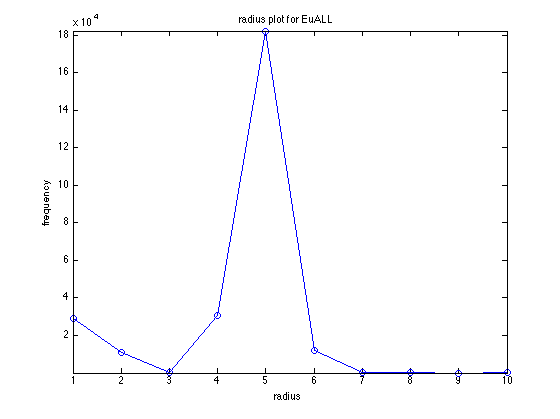
\includegraphics[width=0.8\textwidth]{FIG/t4_email.png} 
\caption{EU Email Communication }
\label{t4:1}
\end{center}
\end{figure}

\begin{figure}[!htbf]
\begin{center}
\begin{tabular}{cc}
     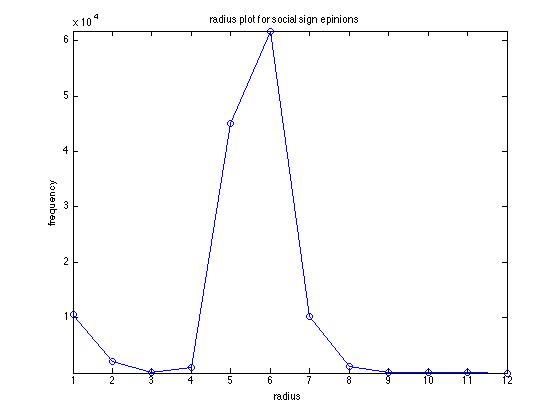
\includegraphics[width=0.8\textwidth]{FIG/t4_epinions.png} 
\end{tabular}
\caption{Epinions social network}
\label{t4:2}
\end{center}
\end{figure}


\begin{figure}[!htbf]
\begin{center}
     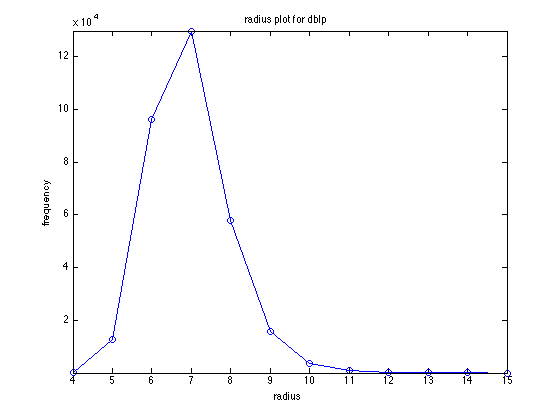
\includegraphics[width=0.8\textwidth]{FIG/t4_dblp.png} 
\caption{DBLP co-authorship network}
\label{t4:3}
\end{center}
\end{figure}


\begin{figure}[!htbf]
\begin{center}
     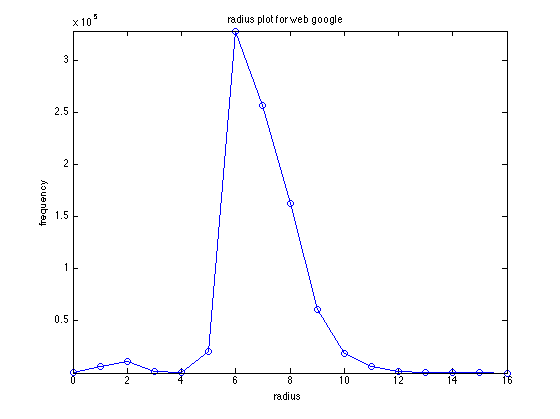
\includegraphics[width=0.8\textwidth]{FIG/t4_google.png} 
\caption{Google Web Graph}
\label{t4:4}
\end{center}
\end{figure}


\begin{figure}[!htbf]
\begin{center}
     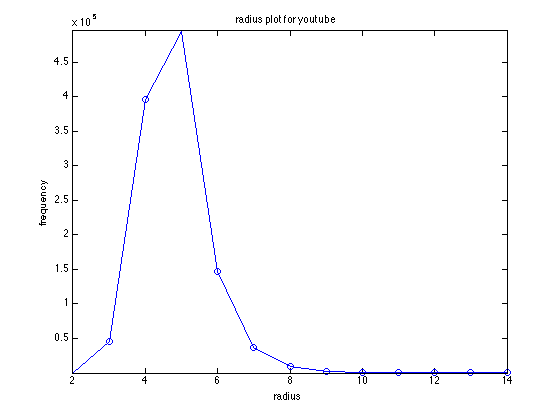
\includegraphics[width=0.8\textwidth]{FIG/t4_youtube.png} 
\caption{Youtube Social Network}
\label{t4:5}
\end{center}
\end{figure}

\begin{figure}[!htbf]
\begin{center}
     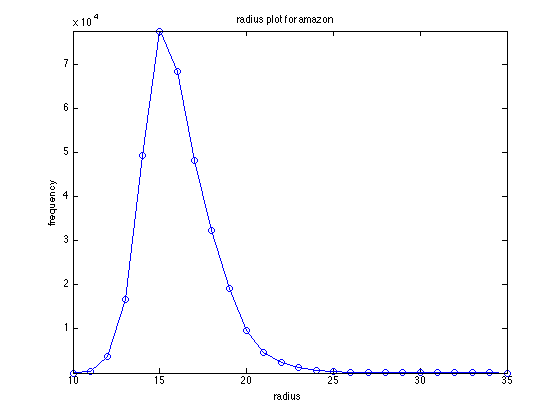
\includegraphics[width=0.8\textwidth]{FIG/t4_amazon.png} 
\caption{Amazon product co-purchasing networkk}
\label{t4:6}
\end{center}
\end{figure}


 
\subsubsection{Observation}
1. Radius Distribution: From the above plot, we find radius distribution of these graphs either tend to be single-modal, for example, EU Email Communication graph in figure \ref{t4:1} and Epinions Social Network in figure \ref {t4:2}, or bi-modal like DBLP co-authorship network in figure \ref{t4:3} and Youtube Social Network in figure \ref{t4:5}.

2. Relationship to the connected component: So why radius tend to be distributed like this, we guess it's somehow related to the connectivity of the graph. Therefore we take a look back to the statistics we got from task3. We find that the graphs that has a single-modal shape radius distribution are fully or almost fully connected. The graphs that has bi-modal radius distribution are not that well connected, For most nodes that appear in the Giant Connected Component(GCC), they tend to have a higher radius value, specifically the smaller radius value it has, the more centric it is in the GCC. On the other hand, The first peak in the radius distribution represent those disconnected components.

\subsubsection{Proof of Correctness}
Since the algorithm we use is an approximate algorithm, it's hard for us to verify the validity of our algorithm accurately. But we still try the algorithm on both small, large and synthetic datasets to demonstrate its validity.  
First we test the algorithm on the synthetic tiny dataset consisting of only 10 nodes and 8 edges. It accurately compute the radius of every node.
 
Then we test our algorithm on small datasets of several thousands of nodes, the experiment result are showed in Table \ref{table:small}, we can see that our algorithm can get a closer estimate of diameter.

\begin{table}[!htbf]
\caption{Radius Experiment on Small Datasets}
\begin{center}
\begin{tabular}{|c|c|c|c|c|}
\hline \hline
dataset & nodes & edges & real diameter & estimated diameter \\
\hline
Enron email network & 36692 & 183831 & 11 & 11 \\
High Energy Physics & 12008 & 118521 & 13 & 12 \\
Advogato Trust Network & 6551 & 51332 & 9 & 9 \\
\hline
\end{tabular}
\end{center}
\label{table:small}
\end{table}%

For large dataset we run in last section, the estimated diameter is still bounded by real diameter, but the estimation is no longer that close. This can be explained by the approximation nature of the algorithm we use. The Flajolet-Martin string we generate for every node is not unique, and as the number of nodes grows larger, the uniqueness of a node that a Flajolet-Martin string can represent is weakened. Therefore, for graph with larger size, the estimation might become less accurate.





